\subsection{梳理:傅里叶变换和傅里叶级数之间的关系}

\begin{figure}[H]
    \centering
    \begin{tabular}{c||c|c}
        \textbf{ } & \textbf{FS} & \textbf{FT} \\
        \hline
        被分析对象 & 周期信号 & 非周期信号 \\
        \hline
        频率定义域 & 离散频率,谐波频率处 & 连续频率,整个频率轴 \\
        \hline
        函数值意义 & 频率分量的数值 & 频率分量的密度值 \\
    \end{tabular}
\end{figure}

\begin{figure}[H]
    \centering
    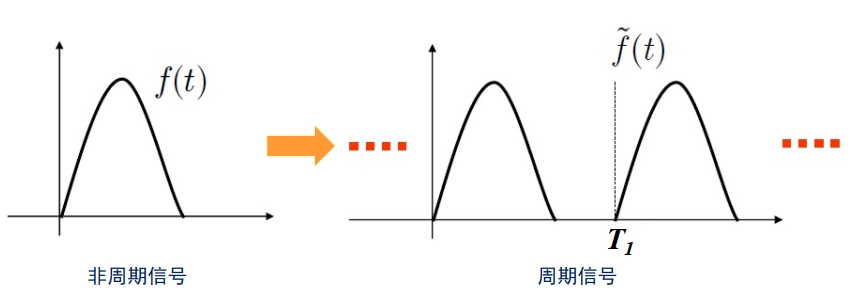
\includegraphics[width = 0.8\textwidth]{chap2/img/fs-ft.png}
    \caption{FS 与 FT 的关系}
    \label{fig:fs-ft}
\end{figure}

后续讨论均基于以上图 \ref{fig:fs-ft}。右侧的周期信号 $\tilde{f}(t)$ 是左侧非周期信号 $f(t)$ 以 $T_1$ 为周期重复的结果。

\subsubsection{现象一:从 FS 到 FT}

\begin{theorem}[FS 与 FT 的关系]
    设有一个定义在 $[0, T_1)$ 上的非周期信号 $f(t)$,
    将其以周期 $T_1$ 重复,得到周期信号 $\tilde{f}(t)$。
    则 $\tilde{f}(t)$ 的 FS 系数 $F_n$ 与 $f(t)$ 的 FT $F(\omega)$ 之间有如下关系:
    \begin{align*}
        F_n = \frac{F(n\omega_1)}{T_1},
    \end{align*}
    其中 $\omega_1 = 2\pi / T_1$。
\end{theorem}

\begin{proof}
    由于
    \begin{align*}
        F_n & = \frac{1}{T_1}\int_{-T_1/2}^{T_1/2}\tilde{f}(t)\mathe^{-\mathi n\omega_1 t}\D{t} \\
        & = \frac{1}{T_1}\int_{-T_1/2}^{T_1/2}f(t)\mathe^{-\mathi n\omega_1 t}\D{t} \\
        & = \frac{1}{T_1}\int_{-\infty}^{+\infty}f(t)\mathe^{-\mathi n\omega_1 t}\D{t},
    \end{align*}
    且 $F(\omega) = \int_{-\infty}^{+\infty}f(t)\mathe^{-\mathi\omega t}\D{t}$,
    因此
    \begin{align*}
        F_n = \frac{F(n\omega_1)}{T_1}.
    \end{align*}
    命题得证。
\end{proof}

以上定理说明,周期信号的第 $n$ 个谐波分量系数 $F_n$,对应频率为 $n\omega_1$,
系数值等于非周期信号 $f(t)$ 的频谱密度函数 $F(\omega)$ 在
频率 $n\omega_1$ 处的函数值除以 $T$。

若以不同的周期对信号 $f(t)$ 进行周期重复,则对这些不同的周期信号,
它们 FS 系数都与信号 $f(t)$ 的 FT 有关!

\begin{definition}[谐波]
    \bd{谐波}是指频率为基波频率的整数倍的辅波或分量。
\end{definition}

\begin{example}[准周期信号的 FT]
    以语音的浊音(元音)和清音(部分辅音)为例。元音都是浊音,是准周期信号,
    一些辅音(除 m、n、l、r 外)是清音,是非周期信号。
    对这两种信号进行频谱分析,可以得到如下结果:
    \begin{itemize}
        \item 辅音
        \begin{figure}[H]
            \centering
            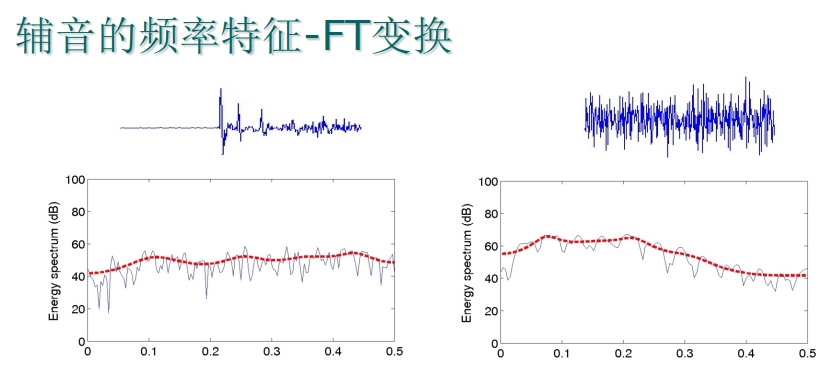
\includegraphics[width = 0.8\textwidth]{chap2/img/consonant.png}
            \caption{辅音信号的频谱}
            \label{fig:consonant}
        \end{figure}
        \begin{itemize}
            \item 辅音无谐波结构
            \item 几乎平坦的谱包络,无明显的共振峰
        \end{itemize}
        \item 元音
            \begin{figure}[H]
                \centering
                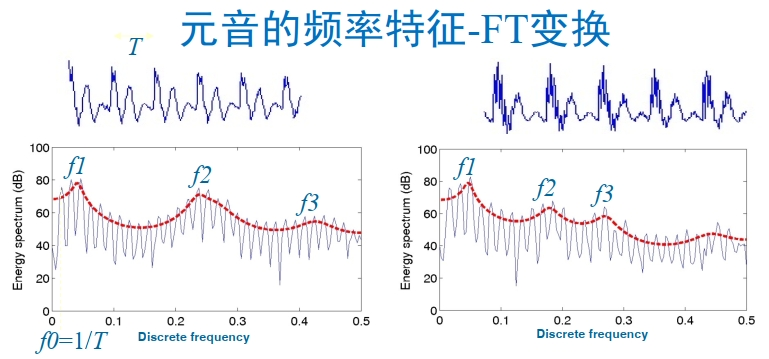
\includegraphics[width = 0.8\textwidth]{chap2/img/vowel.png}
                \caption{元音信号的频谱}
                \label{fig:vowel}
            \end{figure}
            \begin{itemize}
                \item 元音可以清楚地看到信号的周期性
                \item 基频 $f_0 = 1/T$
                \item 具有谐波结构
                \item 谱包络有明显的共振峰
            \end{itemize}
    \end{itemize}
\end{example}

\subsubsection{现象二:FS 与非周期信号}

FS 是函数正交分解的一种,因此它也可用于对非周期信号在特定区间上的一段进行展开(分解)。
若 $f(t)$ 是非周期信号,则分解区间被限制为 $(t_0, t_0 + T_1)$,即 FS 仅在
区间 $(t_0, t_0 + T_1)$ 内成立:

\begin{align*}
    f(t) = \sum_{n = -\infty}^{+\infty} F_n\mathe^{\mathi n\omega_1 t}, \quad t \in (t_0, t_0 + T_1),
\end{align*}
其中 $\omega_1 = 2\pi / T_1$。

\subsubsection{现象三:FT 与周期信号}

\begin{theorem}
    求证:
    \begin{align*}
        \mathcal{F}[\mathe^{\mathi \omega_0 t}] = 2\pi\delta(\omega - \omega_0).
    \end{align*}
    (提示:傅里叶变换无法求解,试试傅里叶逆变换。)
\end{theorem}

\begin{proof}
    由于
    \begin{align*}
        \mathcal{F}^{-1}[2\pi\delta(\omega - \omega_0)] & = \frac{1}{2\pi}\int_{-\infty}^{+\infty}2\pi\delta(\omega - \omega_0)\mathe^{\mathi\omega t}\D{\omega} \\
        & = \int_{-\infty}^{+\infty}\delta(\omega - \omega_0)\mathe^{\mathi\omega t}\D{\omega} \\
        & = \mathe^{\mathi\omega_0 t},
    \end{align*}
    两边同时进行傅里叶变换,得到
    \begin{align*}
        \mathcal{F}[\mathe^{\mathi \omega_0 t}] & = \mathcal{F}[\mathcal{F}^{-1}[2\pi\delta(\omega - \omega_0)]] \\
        & = 2\pi\delta(\omega - \omega_0).
    \end{align*}
    命题得证。
\end{proof}

\begin{example}[余弦信号与正弦信号的 FT]
    利用上述结论,我们可以求解余弦信号和正弦信号的 FT:
    \begin{itemize}
        \item 余弦信号的 FT
            \begin{align*}
                \mathcal{F}[\cos\omega_0t] & = \mathcal{F}\left[\frac{\mathe^{\mathi \omega_0 t} + \mathe^{-\mathi \omega_0 t}}{2}\right] \\
                & = \pi(\delta(\omega - \omega_0) + \delta(\omega + \omega_0)).
            \end{align*}
        \item 正弦信号的 FT
            \begin{align*}
                \mathcal{F}[\sin\omega_0t] & = \mathcal{F}\left[\frac{\mathe^{\mathi \omega_0 t} - \mathe^{-\mathi \omega_0 t}}{2\mathi}\right] \\
                & = \mathi\pi(\delta(\omega + \omega_0) - \delta(\omega - \omega_0)).
            \end{align*}
    \end{itemize}
\end{example}
